\documentclass[12pt]{article}
\usepackage[warn]{mathtext}
\usepackage[T2A]{fontenc}
\usepackage[utf8]{inputenc}
\usepackage[russian]{babel}
\usepackage{amssymb}
\usepackage[left=2.5cm, right=1.5cm, top=2cm, bottom=2cm, bindingoffset=0cm]{geometry}

\usepackage{graphicx}
\graphicspath{{Pictures/}}
\DeclareGraphicsExtensions{.pdf,.png,.jpg}

\usepackage{color}
\usepackage{minted}



\begin{document}

  \begin{titlepage}
    \newpage

    \begin{center}
      Московский Физико-Технический Институт\\
      (Государственный университет)
    \end{center}

    \vspace{8em}

    \begin{center}
      \large Курсовой проект по курсу "Микроконтроллеры"\\
    \end{center}

    %\vspace{1em}

    \begin{center}
      \Large \textsc{\textbf{Метеостанция}}
    \end{center}

    \vspace{6em}

    \begin{center}
      Карцев Вадим, Б01-904\\
      Тяжкороб Ульяна, Б01-909\\
      Янович Максим, Б01-909\\
      Безянова Елизавета, С01-919
    \end{center}


    \vspace{\fill}

    \begin{center}
      Долгопрудный\\
      2021
    \end{center}

  \end{titlepage}



  \section{Описание проекта}

    \subsection{Возможности}
      Собранное устройство позволяет в реальном времени отслеживать параметры
      окружающей среды, такие, как температура, влажность и давление.
      Данные представляются в наиболее популярных величинах измерения.\\
      Кроме того, на базе атмосферного давления устройство умеет определять
      примерную высоту над уровнем моря.\\
      Также устройство отображает уведомления о слишком низкой или высокой
      влажности и уведомления о неисправности сенсора.

    \subsection{Управление}
      Управление устройством осуществляется с помощью одной кнопки, которая
      переключает экраны, отображающие различные категории значений:
      Температура (Temp), Давление (Pressure), Высота (Altitude) и Влажность
      (Humidity).


  \section{Документация}

    \subsection{Используемые модули}
      \begin{itemize}
        \item Arduino Nano (ATMega 328p, 16MHz)
        \item Комбинированный датчик условий окружающей среды BME280
        \item Экран монохромный HX1230
        \item Сенсорная кнопка (цифровая)
      \end{itemize}

    \subsection{Используемые библиотеки}
      \begin{itemize}
        \item U8g2lib.h
        \item Adafruit\_Sensor.h
        \item Adafruit\_BME280.h
      \end{itemize}


  \section{Подключение модулей}

    \begin{minipage}{0.33\textwidth}
      \begin{flushleft}
        Display

        \vspace{0.3cm}

        $CLK \rightarrow D4$\\
        $DIN \rightarrow D5$\\
        $CE \rightarrow D7$\\
        $RST \rightarrow D8$\\

      \end{flushleft}
    \end{minipage}
    \begin{minipage}{0.33\textwidth}
      \begin{flushleft}
        BME280 Sensor

        \vspace{0.3cm}

        $SCL \rightarrow D13$\\
        $SDA \rightarrow D11$\\
        $SCB \rightarrow D10$\\
        $SDO \rightarrow D12$\\

      \end{flushleft}
    \end{minipage}
    \begin{minipage}{0.33\textwidth}
      \begin{flushleft}
        Touch Button

        \vspace{0.3cm}

        $I/O \rightarrow D2$

      \end{flushleft}
    \end{minipage}

  \newpage
  \section{Фотографии проекта}

    \subsection{Устройство}
      \begin{figure}[h]
        \center{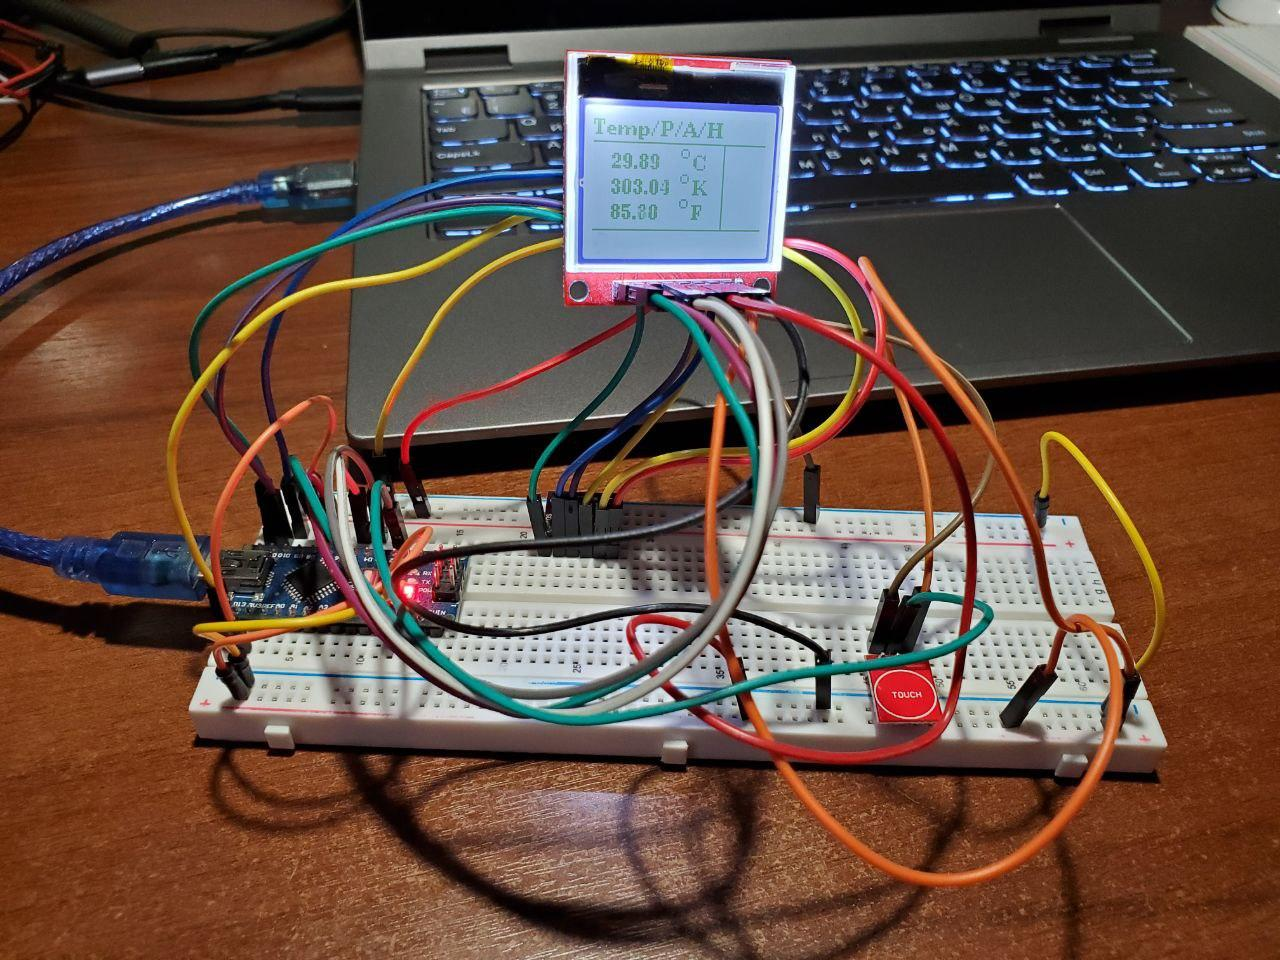
\includegraphics[width=1\linewidth]{project.jpg}}
        \label{ris:image1}
      \end{figure}

    \subsection{Интерфейс}
      \begin{figure}[h]
        \begin{minipage}[h]{0.24\linewidth}
          \center{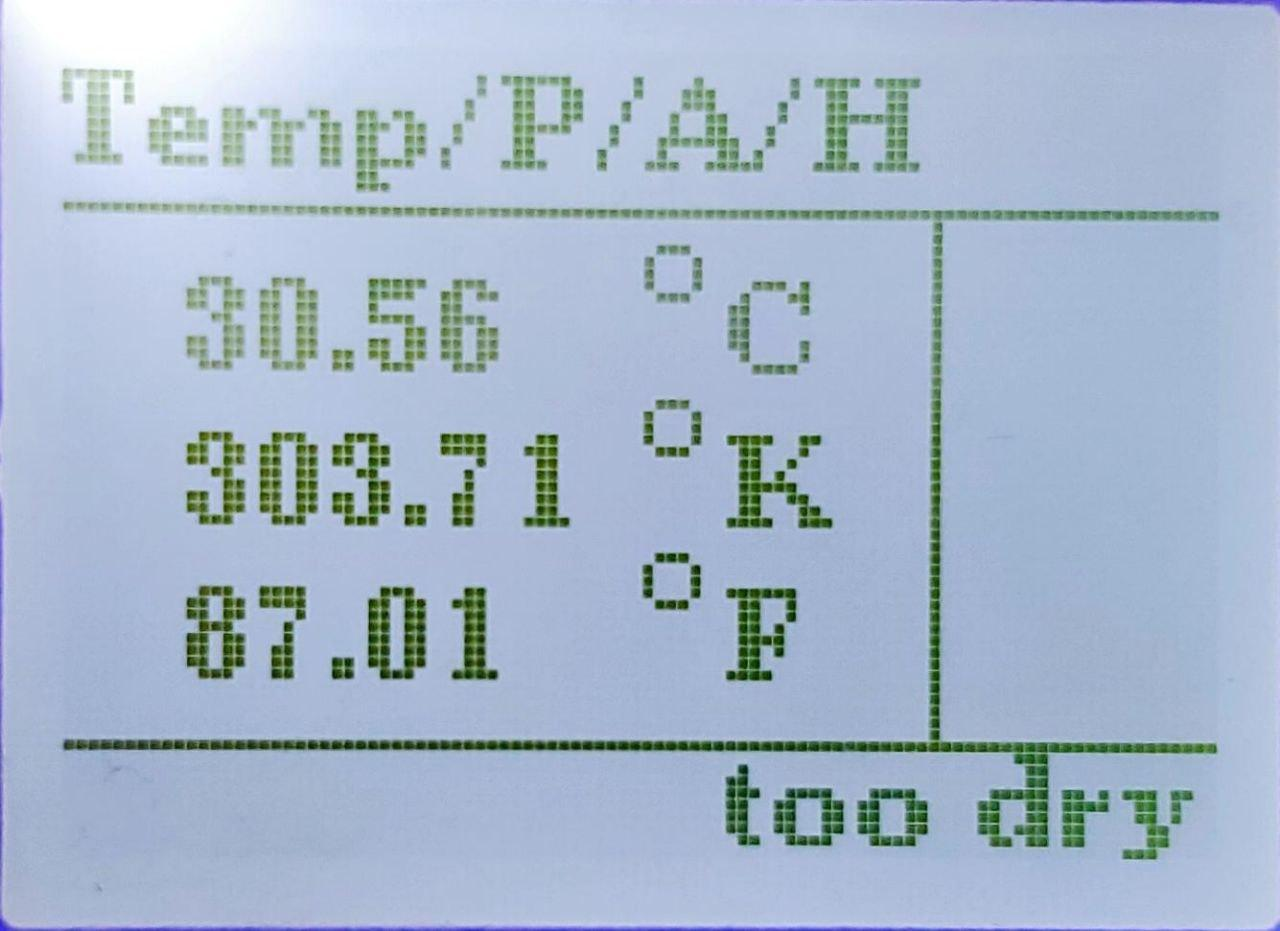
\includegraphics[width=1\linewidth]{screen1.jpg} \\ Температура}
        \end{minipage}
        \hfill
        \begin{minipage}[h]{0.24\linewidth}
          \center{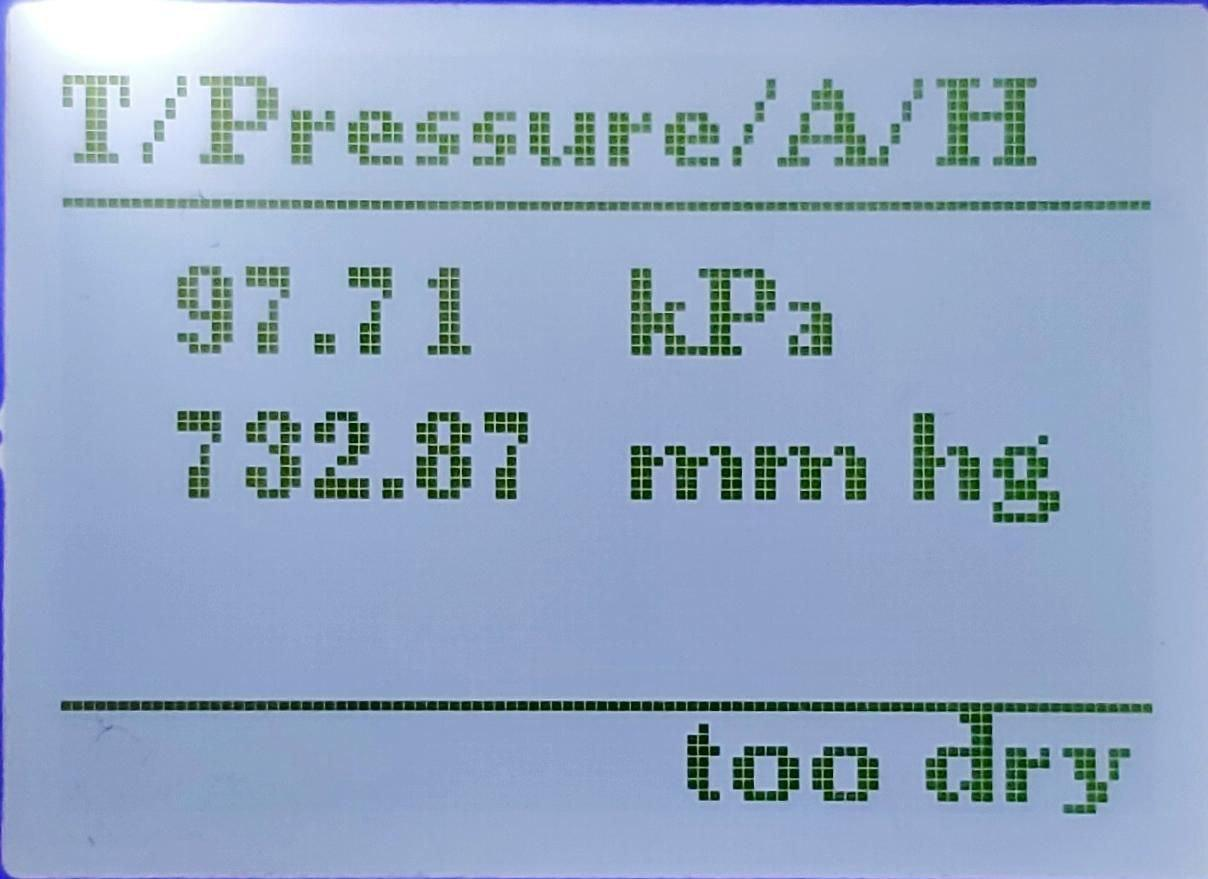
\includegraphics[width=1\linewidth]{screen2.jpg} \\ Давление}
        \end{minipage}
        \hfill
        \begin{minipage}[h]{0.24\linewidth}
          \center{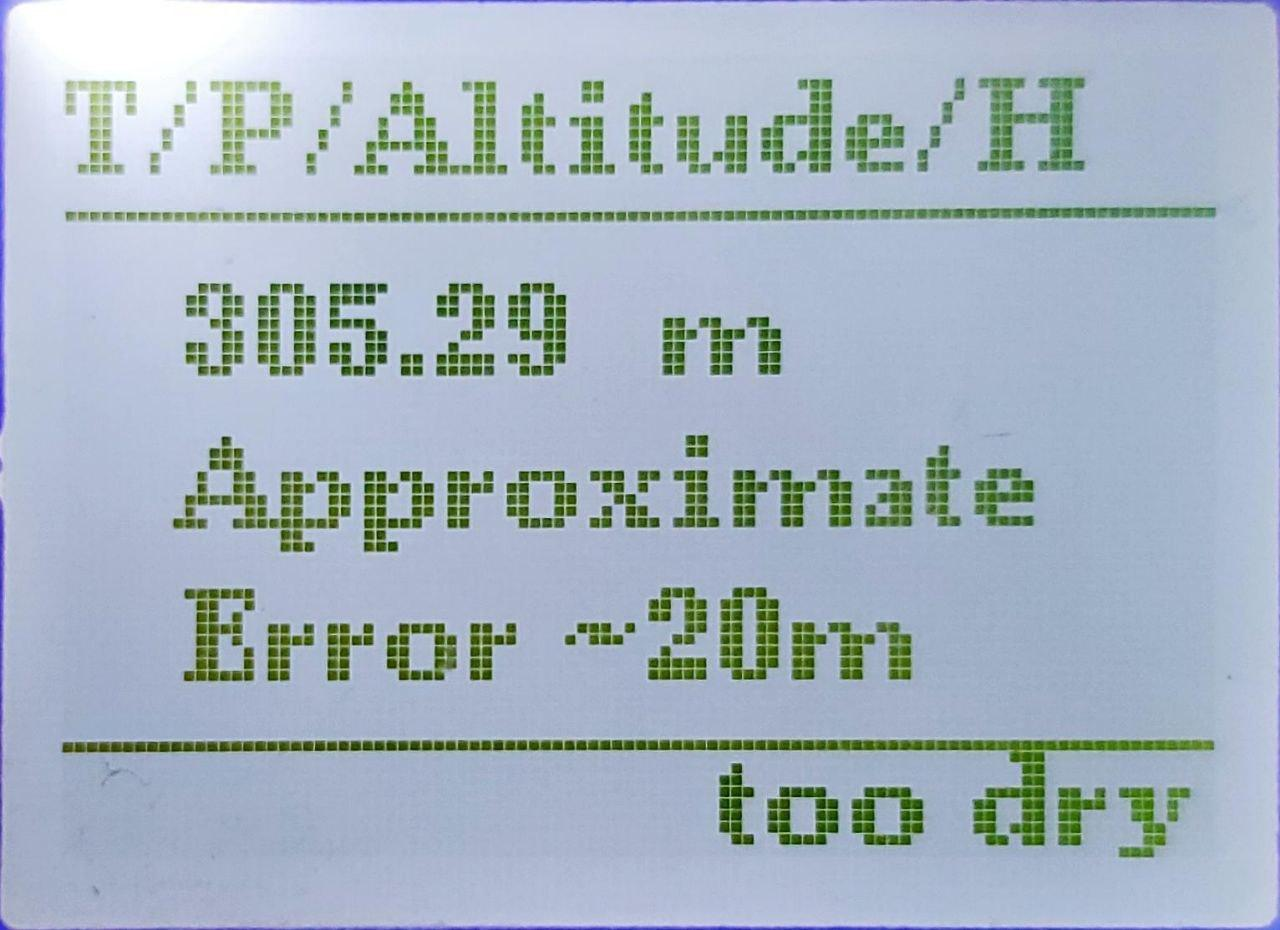
\includegraphics[width=1\linewidth]{screen3.jpg} \\ Высота}
        \end{minipage}
        \hfill
        \begin{minipage}[h]{0.24\linewidth}
          \center{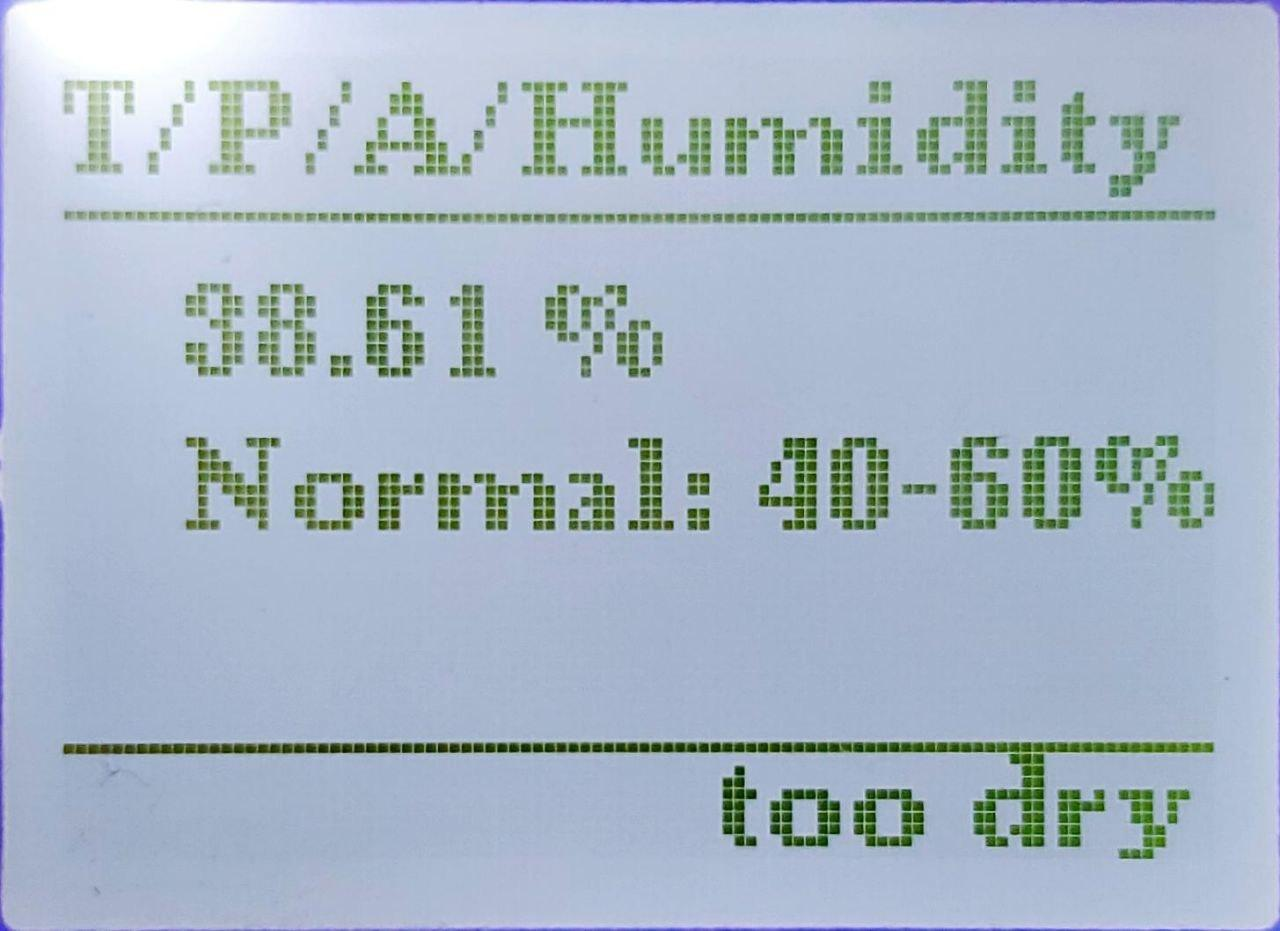
\includegraphics[width=1\linewidth]{screen4.jpg} \\ Влажность}
        \end{minipage}
        \label{ris:image2}
      \end{figure}

  \newpage
  \section{Исходный код проекта}
    \begin{minted}[fontsize=\footnotesize, linenos]{c++}
      #include <U8g2lib.h>
      #include <Adafruit_Sensor.h>
      #include <Adafruit_BME280.h>

      // define pins for sensor   (VCC -> 3V3, GND -> GND)
      #define BME_SCK   13      // SCL pin on sensor
      #define BME_MISO  12      // SDO pin on sensor
      #define BME_MOSI  11      // SDA pin on sensor
      #define BME_CS    10      // SCB pin on sensor

      // define pins for display  (VCC -> 5V, BL -> 3V3, GND -> GND)
      #define DISPLAY_CLOCK 4   // CLK pin on display
      #define DISPLAY_DATA  5   // DIN pin on display
      #define DISPLAY_CS    7   // CE pin on display
      #define DISPLAY_RESET 8   // RST pin on display

      // define pins for key   (5V -> 5V, GND -> GND)
      #define TOUCH_KEY 2

      #define SEALEVELPRESSURE_HPA (1013.25)

      Adafruit_BME280 sensor(BME_CS, BME_MOSI, BME_MISO, BME_SCK);
      U8G2_HX1230_96X68_F_3W_SW_SPI display(U8G2_R0, DISPLAY_CLOCK, DISPLAY_DATA, DISPLAY_CS, DISPLAY_RESET);


      void sensorError();
      void drawFrame(int frame);
      int checkKey();
      int next(int frame);


      int FrameNumber = 0;
      int Time_from_last_update = 0;
      int SensorError = 0;


      void setup(void)
      {
        display.begin();

        bool status;
        status = sensor.begin();
        if (!status) SensorError = 1;
        delay(100); //Sensor bootup
        drawFrame(FrameNumber);
      }

      void loop(void)
      {
        int frame = FrameNumber;
        int command = checkKey();

        if (command == 1) FrameNumber = next(FrameNumber);

        if ((frame != FrameNumber) or (Time_from_last_update > 1000))
        {
          Time_from_last_update = 0;
          drawFrame(FrameNumber);
        }

        delay(1);
        Time_from_last_update++;
      }


      void drawFrame(int frame)
      {
        display.clearBuffer();
        display.setFont(u8g2_font_ncenB08_tr);

        display.drawLine(0,13,96,13);
        display.drawLine(0,58,96,58);

        drawBar();

        switch(frame)
        {
          case(0):
          {
            display.drawStr(0, 10, "Temp/P/A/H");
            float temp_celsius = sensor.readTemperature();
            display.setCursor(10, 27);
            display.print(temp_celsius, 2); // Temperature in Celsius
            display.drawCircle(50, 18, 2);
            display.drawStr(52, 27, " C");
            display.setCursor(10, 40);
            display.print(temp_celsius + 273.15, 2); // Temperature in Kelvins
            display.drawCircle(50, 31, 2);
            display.drawStr(52, 40, " K");
            display.setCursor(10, 53);
            display.print(temp_celsius * 1.8 + 32, 2); // Temperature in Farengeith
            display.drawCircle(50, 44, 2);
            display.drawStr(52, 53, " F");
            display.drawLine(72,13,72,58);
            break;
          }
          case(1):
          {
            display.drawStr(0, 10, "T/Pressure/A/H");
            float pressure_pa = sensor.readPressure();
            display.setCursor(10, 27);
            display.print(pressure_pa / 1000.0F, 2);
            display.drawStr(50, 27, "kPa");
            display.setCursor(10, 40);
            display.print(pressure_pa / 133.332, 2);
            display.drawStr(50, 40, "mm hg");
            break;
          }
          case(2):
          {
            display.drawStr(0, 10, "T/P/Altitude/H");
            display.setCursor(10, 27);
            display.print(sensor.readAltitude(SEALEVELPRESSURE_HPA),2);
            display.drawStr(50, 27, "m");
            display.drawStr(10, 40, "Approximate");
            display.drawStr(10, 53, "Error ~20m");
            break;
          }
          case(3):
          {
            display.drawStr(0, 10, "T/P/A/Humidity");
            display.setCursor(10, 27);
            display.print(sensor.readHumidity(), 2);
            display.drawStr(40, 27, "%");
            display.drawStr(10, 40, "Normal: 40-60%");
            break;
          }
        }

        display.sendBuffer();
      }


      int checkKey()
      {
        int command = 0;

        if(digitalRead(TOUCH_KEY))
        {
          command = 1;
          while(digitalRead(TOUCH_KEY));
        }

        return command;
      }


      int next(int frame)
      {
        int NewFrame = frame + 1;
        if(NewFrame > 3) NewFrame = 0;
        return NewFrame;
      }


      void drawBar()
      {
        if(SensorError) display.drawStr(0, 67, "err");
        if(sensor.readHumidity() < 40) display.drawStr(55, 67, "too dry");
        else if (sensor.readHumidity() > 60) display.drawStr(55, 67, "too wet");
      }


      //end;
    \end{minted}



\end{document}
